%begin---------------------Settings---------------------------%
\documentclass[12pt,a4paper,UTF8]{article}
\usepackage{geometry}
	\geometry{left=2cm,right=2cm,top=3.2cm,bottom=2.8cm}
\usepackage{amsmath,paralist,enumitem,booktabs,multirow,graphicx,subfig,setspace,listings,lastpage}
\usepackage[colorlinks,
            linkcolor=blue,       
            anchorcolor=blue,  
            citecolor=blue,       
            ]{hyperref}
	\setlength{\parindent}{2em}
	\lstset{language=Python}
\usepackage{fancyhdr}
	\pagestyle{fancy}
	\lhead{C10}
	\rhead{SUPPLEMENTARY INFORMATION}
	\cfoot{Page \thepage/\pageref{LastPage}}
	\rfoot{\today}
	\renewcommand{\headrulewidth}{0.4pt}
	\renewcommand{\theenumi}{(\arabic{enumi})}

\usepackage[figuresright]{rotating}

\renewcommand{\thefigure}{S\arabic{figure}}
\renewcommand{\thetable}{S\arabic{table}}
%end---------------------Settings---------------------------%



%%%%%%%%%%%%%%%%%%%%%%%%%%%%%%%%%%%%%%%%%%%%%%%%%%%%%%%%%%
%%%%%%%%%%%%%%%%%%%%%%%%%Document%%%%%%%%%%%%%%%%%%%%%%%%%%
%%%%%%%%%%%%%%%%%%%%%%%%%%%%%%%%%%%%%%%%%%%%%%%%%%%%%%%%%%


\begin{document}
%begin---------------------Infor and Catalog---------------------------%

\begin{center}
\LARGE\textbf{C7 SLM-based optical experiment}

\vspace{0.5em}
\large{SUPPLEMENTARY INFORMATION}
\end{center}

\noindent
\textbf{Experimenter:} Zweig, Wong 20980066 \\
\textbf{Participant:} Runbing Mo 20980131 \\
\textbf{Date:} 2022.06


\tableofcontents
\newpage
%end---------------------Infor and Catalog---------------------------%

%begin---------------------Materials and instruments---------------------------%
\section{Materials and instruments}
\begin{table}[htbp]
    \centering
    \caption{\textbf{Materials and instruments}}
        \begin{tabular}{llll}
            \toprule
            Name &Total &Model and parameters \\
            \midrule
            Transmissive Spatial light modulator	&1	&$RL-SLM-T1$, $26.0\mu m$    \\    
            CCD	&1	&$MER-310-12UC$, $3.2 \mu m$    \\
            Laser	&1	&$GP3-CC311-1-0.035-G650-2mWF-3B$    \\  
            Power meter &1	&$GPM100USB$    \\
            Optical elements &/	&/    \\
            \bottomrule
        \end{tabular}
\end{table}	
%end---------------------Materials and instruments---------------------------%

%begin---------------------Exp.1---------------------------%

\section{Exp.1 Distortion of the convex lens imaging system}
    \subsection{Main parameters}
    \begin{table}[htbp]
        \centering
        \caption{\textbf{Parameters}}
        \label{tab.1.0}
            \begin{tabular}{ll}
                \toprule
                Item &parameters  \\
                \midrule
                Checker board resolution & $1024 \times 768$ \\
                Grids of Checker A & $8 \times 6$  \\
                Grids of Checker B & $64 \times 48$  \\
                \bottomrule
            \end{tabular}
    \end{table}	

    \subsection{Supplementary data and figure}
    Tab. \ref{tab.1.1} shows details of distortions in different systems.
    
    $\beta$ is the amplification, $s_1$ is the object distance, $s_2$ is the image distance,
    $g$ represents the number of grids of sampling points apart from each other, $p$ represents the coordinates of the sampling points, 
    $h_1$ is the ideal image height, $h_2$ is the actual image height, $dh$ is the height difference.
    $q$ is the relative distortion, $\theta$ is the optical angle.
    All distance were measured in $\mu m$.
    
    Data are also available in our repository.

    \begin{sidewaystable}[htbp]
        \centering
        \caption{\textbf{Details of distortions in different systems}}
        \label{tab.1.1}
        \resizebox{\columnwidth}{!}{
            \begin{tabular}{llllllllllllllllllllllllllllllll}
            \toprule
            Lab & Checker &   $f$ &  $\beta$ &  $s_1$ &     $s_2$ &  $X_g$ &  $Y_g$ &  $XY_g$ &  $Center_xp$ &  $Center_yp$ &  $X_xp$ &  $Y_yp$ &  $XY_xp$ &  $XY_yp$ &     $X_{h1}$ &     $Y_{h1}$ &   $XY_{h1}x$ &   $XY_{h1}y$ &   $X_{h2}$ &   $Y_{h2}$ &  $XY_{h2}x$ &  $XY_{h2}y$ &     $X_{dh}$ &     $Y_{dh}$ &   $XY_{dh}x$ &   $XY_{dh}y$ &     $X_q$ &     $Y_q$ &   $XY_qx$ &   $XY_qy$ &     $\theta$ \\
            \midrule
                150\_4 &       A & 150 & 0.250 & 750 & 187.50 &    2 &    2 &   1.5 &         984 &         706 &   1505 &    179 &    1374 &     324 & 1664.000 & 1664.000 & 1248.000 & 1248.000 & 1667.2 & 1686.4 &  1248.0 &  1222.4 &    3.200 &   22.400 &    0.000 &  -25.600 &   0.19\% &   1.35\% &   0.00\% &  -2.05\% &  2.218667 \\
                70\_4 &       A &  70 & 0.250 & 350 &  87.50 &    2 &    2 &   1.5 &        1089 &         752 &   1662 &    177 &    1520 &     321 & 1664.000 & 1664.000 & 1248.000 & 1248.000 & 1833.6 & 1840.0 &  1379.2 &  1379.2 &  169.600 &  176.000 &  131.200 &  131.200 &  10.19\% &  10.58\% &  10.51\% &  10.51\% &  4.754286 \\
                50\_4 &       A &  50 & 0.250 & 250 &  62.50 &    2 &    2 &   1.5 &        1085 &         767 &   1682 &    208 &    1532 &     337 & 1664.000 & 1664.000 & 1248.000 & 1248.000 & 1910.4 & 1788.8 &  1430.4 &  1376.0 &  246.400 &  124.800 &  182.400 &  128.000 &  14.81\% &   7.50\% &  14.62\% &  10.26\% &  6.656000 \\
                70\_2 &       A &  70 & 0.500 & 210 & 105.00 &    1 &    1 &   1.0 &        1054 &         830 &   1556 &    320 &    1562 &     304 & 1664.000 & 1664.000 & 1664.000 & 1664.000 & 1606.4 & 1632.0 &  1625.6 &  1683.2 &  -57.600 &  -32.000 &  -38.400 &   19.200 &  -3.46\% &  -1.92\% &  -2.31\% &   1.15\% &  7.923810 \\
                70\_6 &       A &  70 & 0.166 & 490 &  81.64 &    2 &    2 &   1.5 &        1061 &         690 &   1466 &    315 &    1367 &     391 & 1104.896 & 1104.896 &  828.672 &  828.672 & 1296.0 & 1200.0 &   979.2 &   956.8 &  191.104 &   95.104 &  150.528 &  128.128 &  17.30\% &   8.61\% &  18.16\% &  15.46\% &  2.246604 \\
            48x64\_2X &       B &  70 & 2.000 & 210 & 105.00 &    2 &    2 &   1.5 &         977 &         734 &   1541 &    171 &    1393 &     314 & 1664.000 & 1664.000 & 1248.000 & 1248.000 & 1804.8 & 1801.6 &  1331.2 &  1344.0 &  140.800 &  137.600 &   83.200 &   96.000 &   8.46\% &   8.27\% &   6.67\% &   7.69\% & 31.695238 \\
            48x64\_4X &       B &  70 & 4.000 & 350 &  87.50 &    1 &    1 &   1.0 &        1071 &         683 &   1459 &    301 &    1459 &     301 & 1664.000 & 1664.000 & 1664.000 & 1664.000 & 1241.6 & 1222.4 &  1241.6 &  1222.4 & -422.400 & -441.600 & -422.400 & -441.600 & -25.38\% & -26.54\% & -25.38\% & -26.54\% & 76.068571 \\
            \bottomrule
            \end{tabular}}
    \end{sidewaystable}	
    
    
    


    \subsection{Question}
        \subsubsection{Which types of spatial light modulator is adopted?}
        As introduced in the thesis, SLM we used in this experiment is transmissive twisted nematic liquid-crystal spatial light modulator (TTNLC-SLM) controlled by voltage. 
        \subsubsection{For the same $\beta$, why distortion in shrinking system is greater than the amplifying system?}
        As explained in the thesis, the distortion is determined by the "off-axis" degree, which could be represented by the optical angle $\theta = \frac{\beta Y}{s_2}$.
        Theoretically, comparing to the amplifying system, the image distance in shrinking system is smaller, thus the $theta$ is greater, the distortion is greater.
        However, in our experiments, we found that the distortions in shrinking system are smaller than the amplifying system.
        We hypothesize that this may be caused by the measuring error as stated in the limitation.
        
        \begin{enumerate}[label=\arabic*.]
            \item 
        \end{enumerate}
        \subsubsection{ }
        \begin{enumerate}[label=\arabic*.]
            \item 
        \end{enumerate}

% %end---------------------Exp.1---------------------------%

% %begin---------------------Exp.2---------------------------%

\section{Exp.2 Optical information processing}

    \subsection{Question}
        \subsubsection{Difference between diffraction patterns of real 1D grating and SLM loaded with 1D grating image. Explain the phenomena of the diffraction patterns based on Abbe's theory of image formation.}
        This has been explained in details in the thesis. In brief, the difference, that is, additional spots in vertical orientation, 
        is caused by the gap between pixels of the SLM, which is opaque and will lead to extra diffraction effects in vertical orientation.

        Explanation of the phenomena is also covered in the thesis.
        \subsubsection{Use Abbe's theory of image formation to explain the limitation of resolving power of the microscope}
        According to Abbe's theory of image formation, the image is formed by interference of beams coming from the Fourier plain, 
        and every spot on the Fourier plain carry detail information about the image. 
        Because the size of the aperture of the microscope is limited, there must be some spots of high order failing to pass through the aperture,
        which will lead to loss of detail information, and the quality of the image is limited.
        If we continually increase the amplification, the spots on the Fourier plain will be more and more sparse, thus more spots are blocked due to the limited size of the aperture, and the quality of the image will be greatly impacted.

        Thus, the resolving power is limited unless we continually increase the size of the aperture, which is usually unpractical.

% %end---------------------Exp.2---------------------------%

% %begin---------------------Exp.3---------------------------%

\section{Exp.3 }
    \subsection{Reflection question}
        \subsubsection{Factors that impact the effects of the quality of hologram}
        \begin{enumerate}[label=\arabic*.]
            \item Correct relationship between object and reference beams.        
            \item Stability and characteristics of the holographic table used.
            \item Proper fixing of all elements of the system.
            \item Characteristics of the surface of the object to holography.
            \item Stability of lasers used.
        \end{enumerate}
        
        \subsubsection{Code for computational holography and digital holography}
        Codes are available in our Github repository. Here we only provide the core part of the codes.
        Code of computational holography and example are shown in Fig. \ref{fig.1}. 
        Code of digital holography and example are shown in Fig. \ref{fig.2}.
        We specially thank \href{https://github.com/JackHCC/Computer-Generated-Hologram}{@JackHCC} and 
        \href{https://github.com/OptoManishK/Digital_Holography}{@OptoManishK} for their inspiration.

        \begin{figure}[htbp]
            \centering
            \subfloat[Code (GS algorithm)]{
            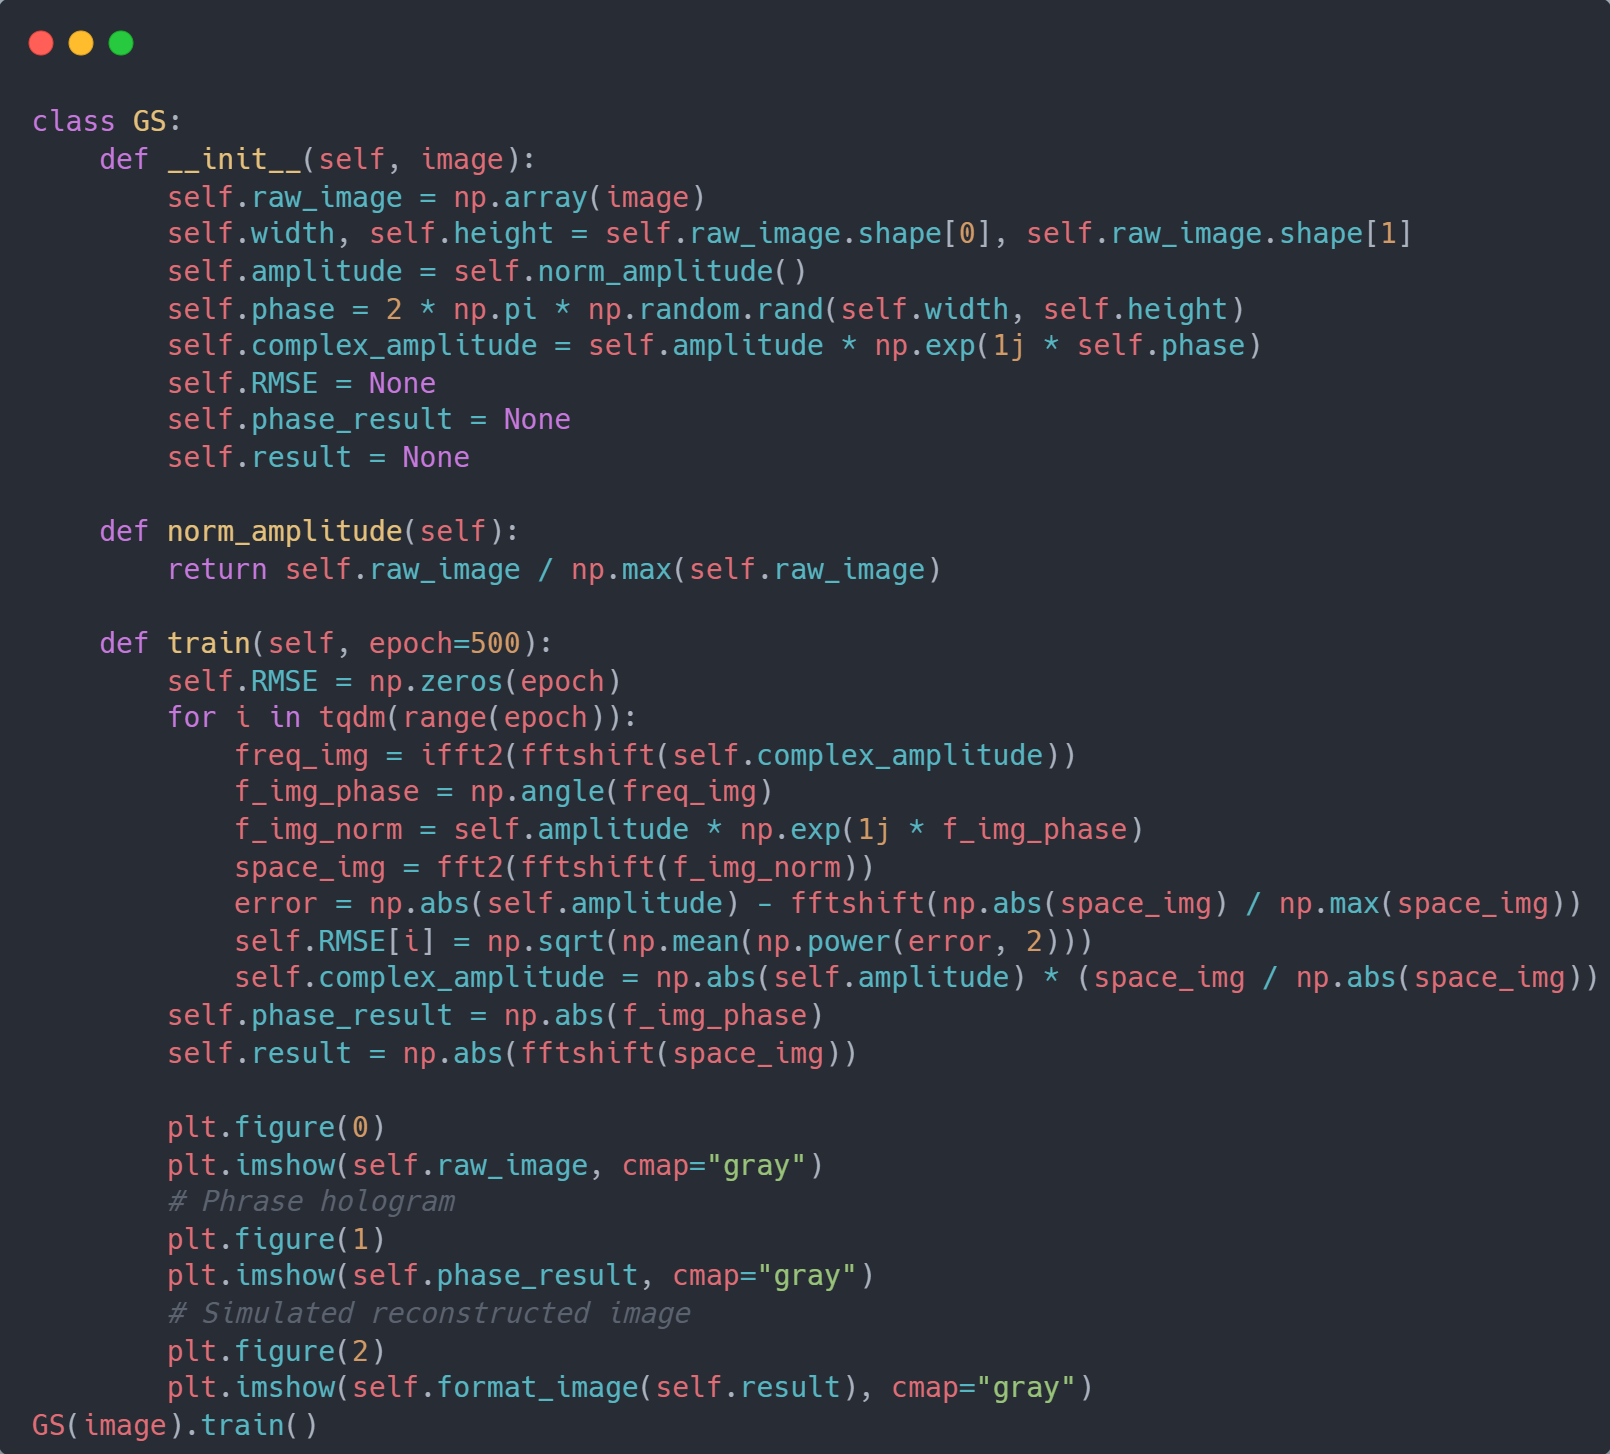
\includegraphics[width=0.4\textwidth]{attachments/Code-comp.png}
            }
            \subfloat[Raw image]{
            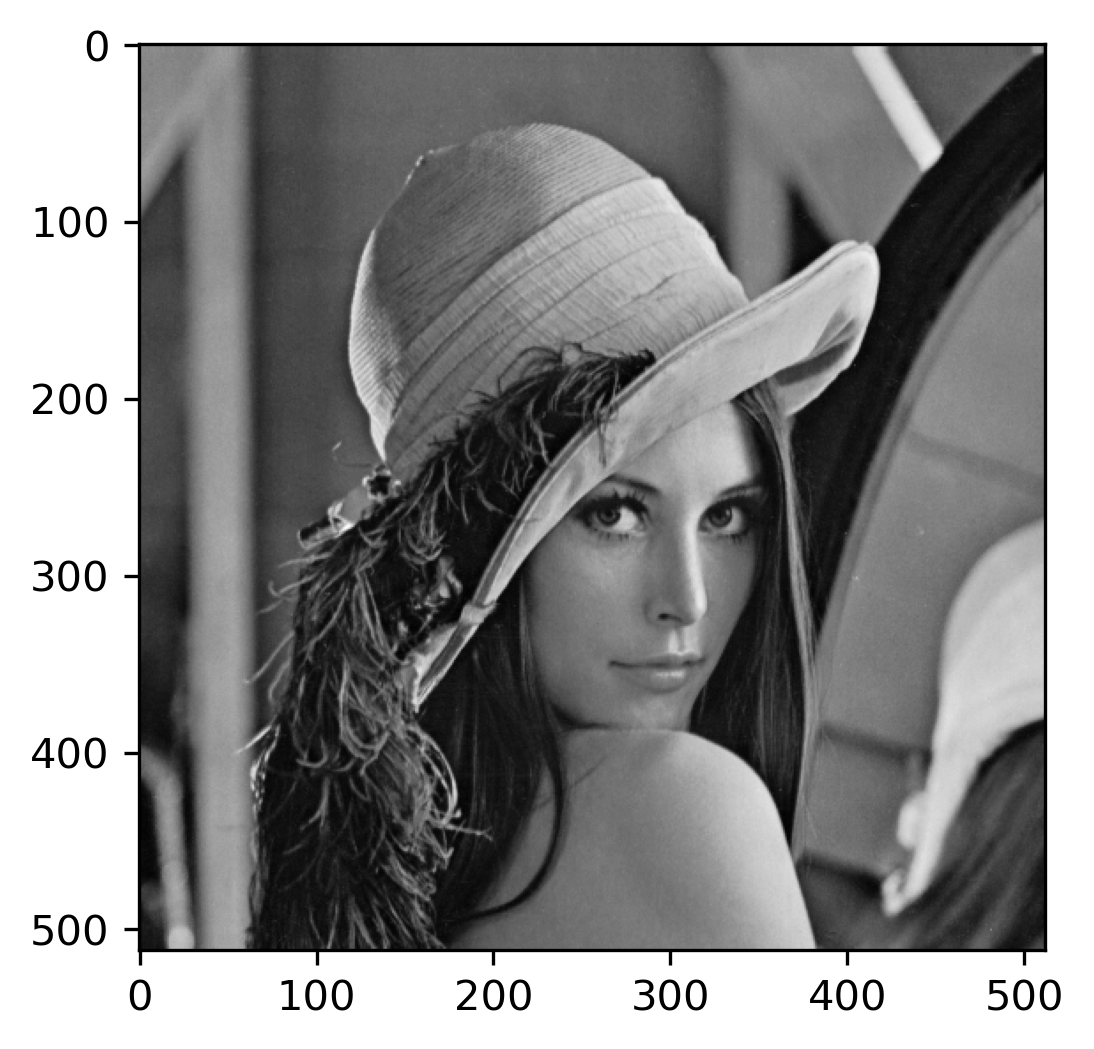
\includegraphics[width=0.4\textwidth]{attachments/lena_raw.png}
            }

            \subfloat[Hologram]{
            \includegraphics[width=0.4\textwidth]{attachments/lena_phrase.png}
            }
            \subfloat[Simulated reconstructed image]{
            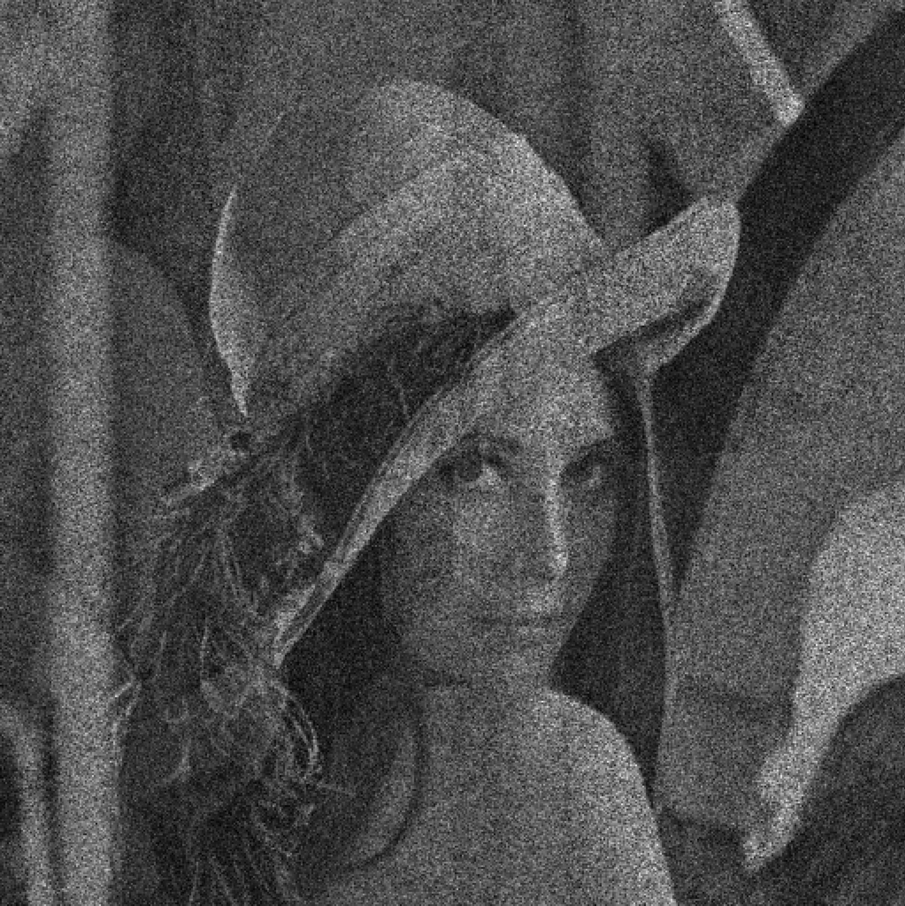
\includegraphics[width=0.4\textwidth]{attachments/lena_reconstructed_sim.png}
            }
            \label{fig.1}
            \caption{\textbf{Computational holography}}
        \end{figure}

        \begin{figure}[htbp]
            \centering
            \subfloat[Code]{
            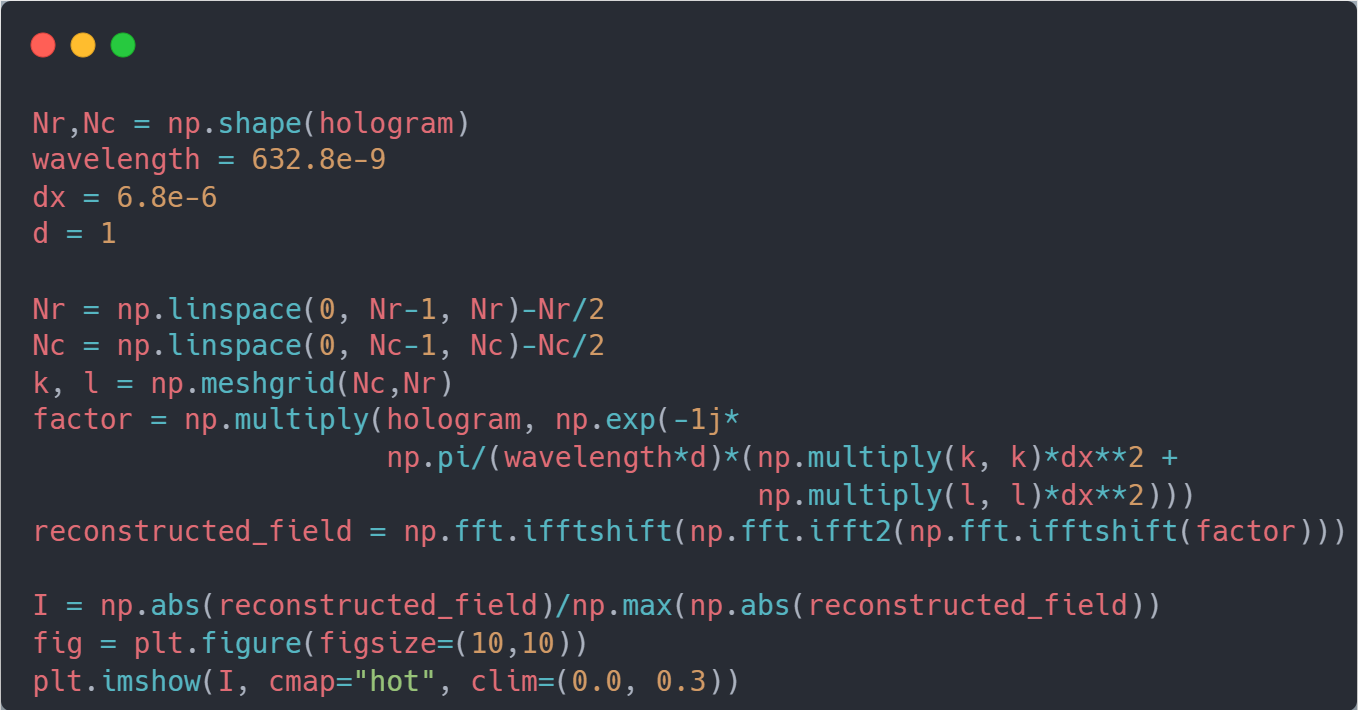
\includegraphics[width=0.3\textwidth]{attachments/Code-digital.png}
            }
            \subfloat[Hologram]{
            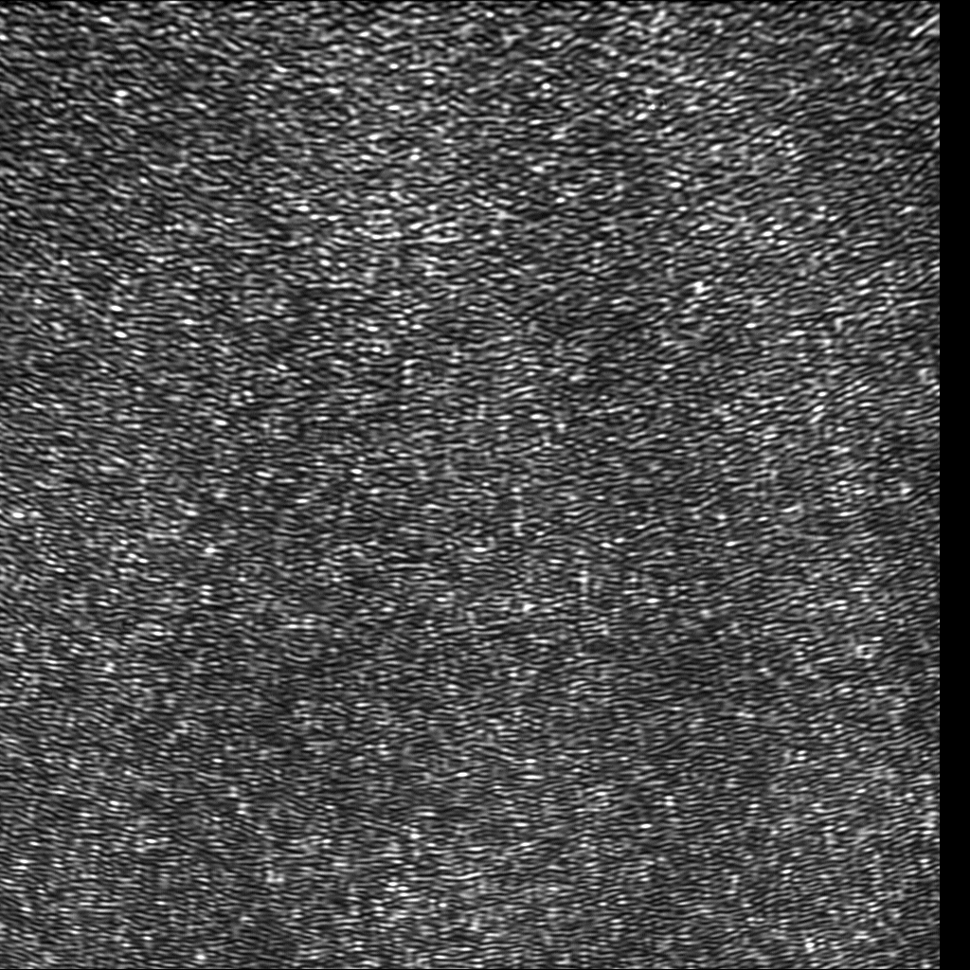
\includegraphics[width=0.3\textwidth]{attachments/dice_holo.png}
            }
            \subfloat[Digital reconstructed image]{
            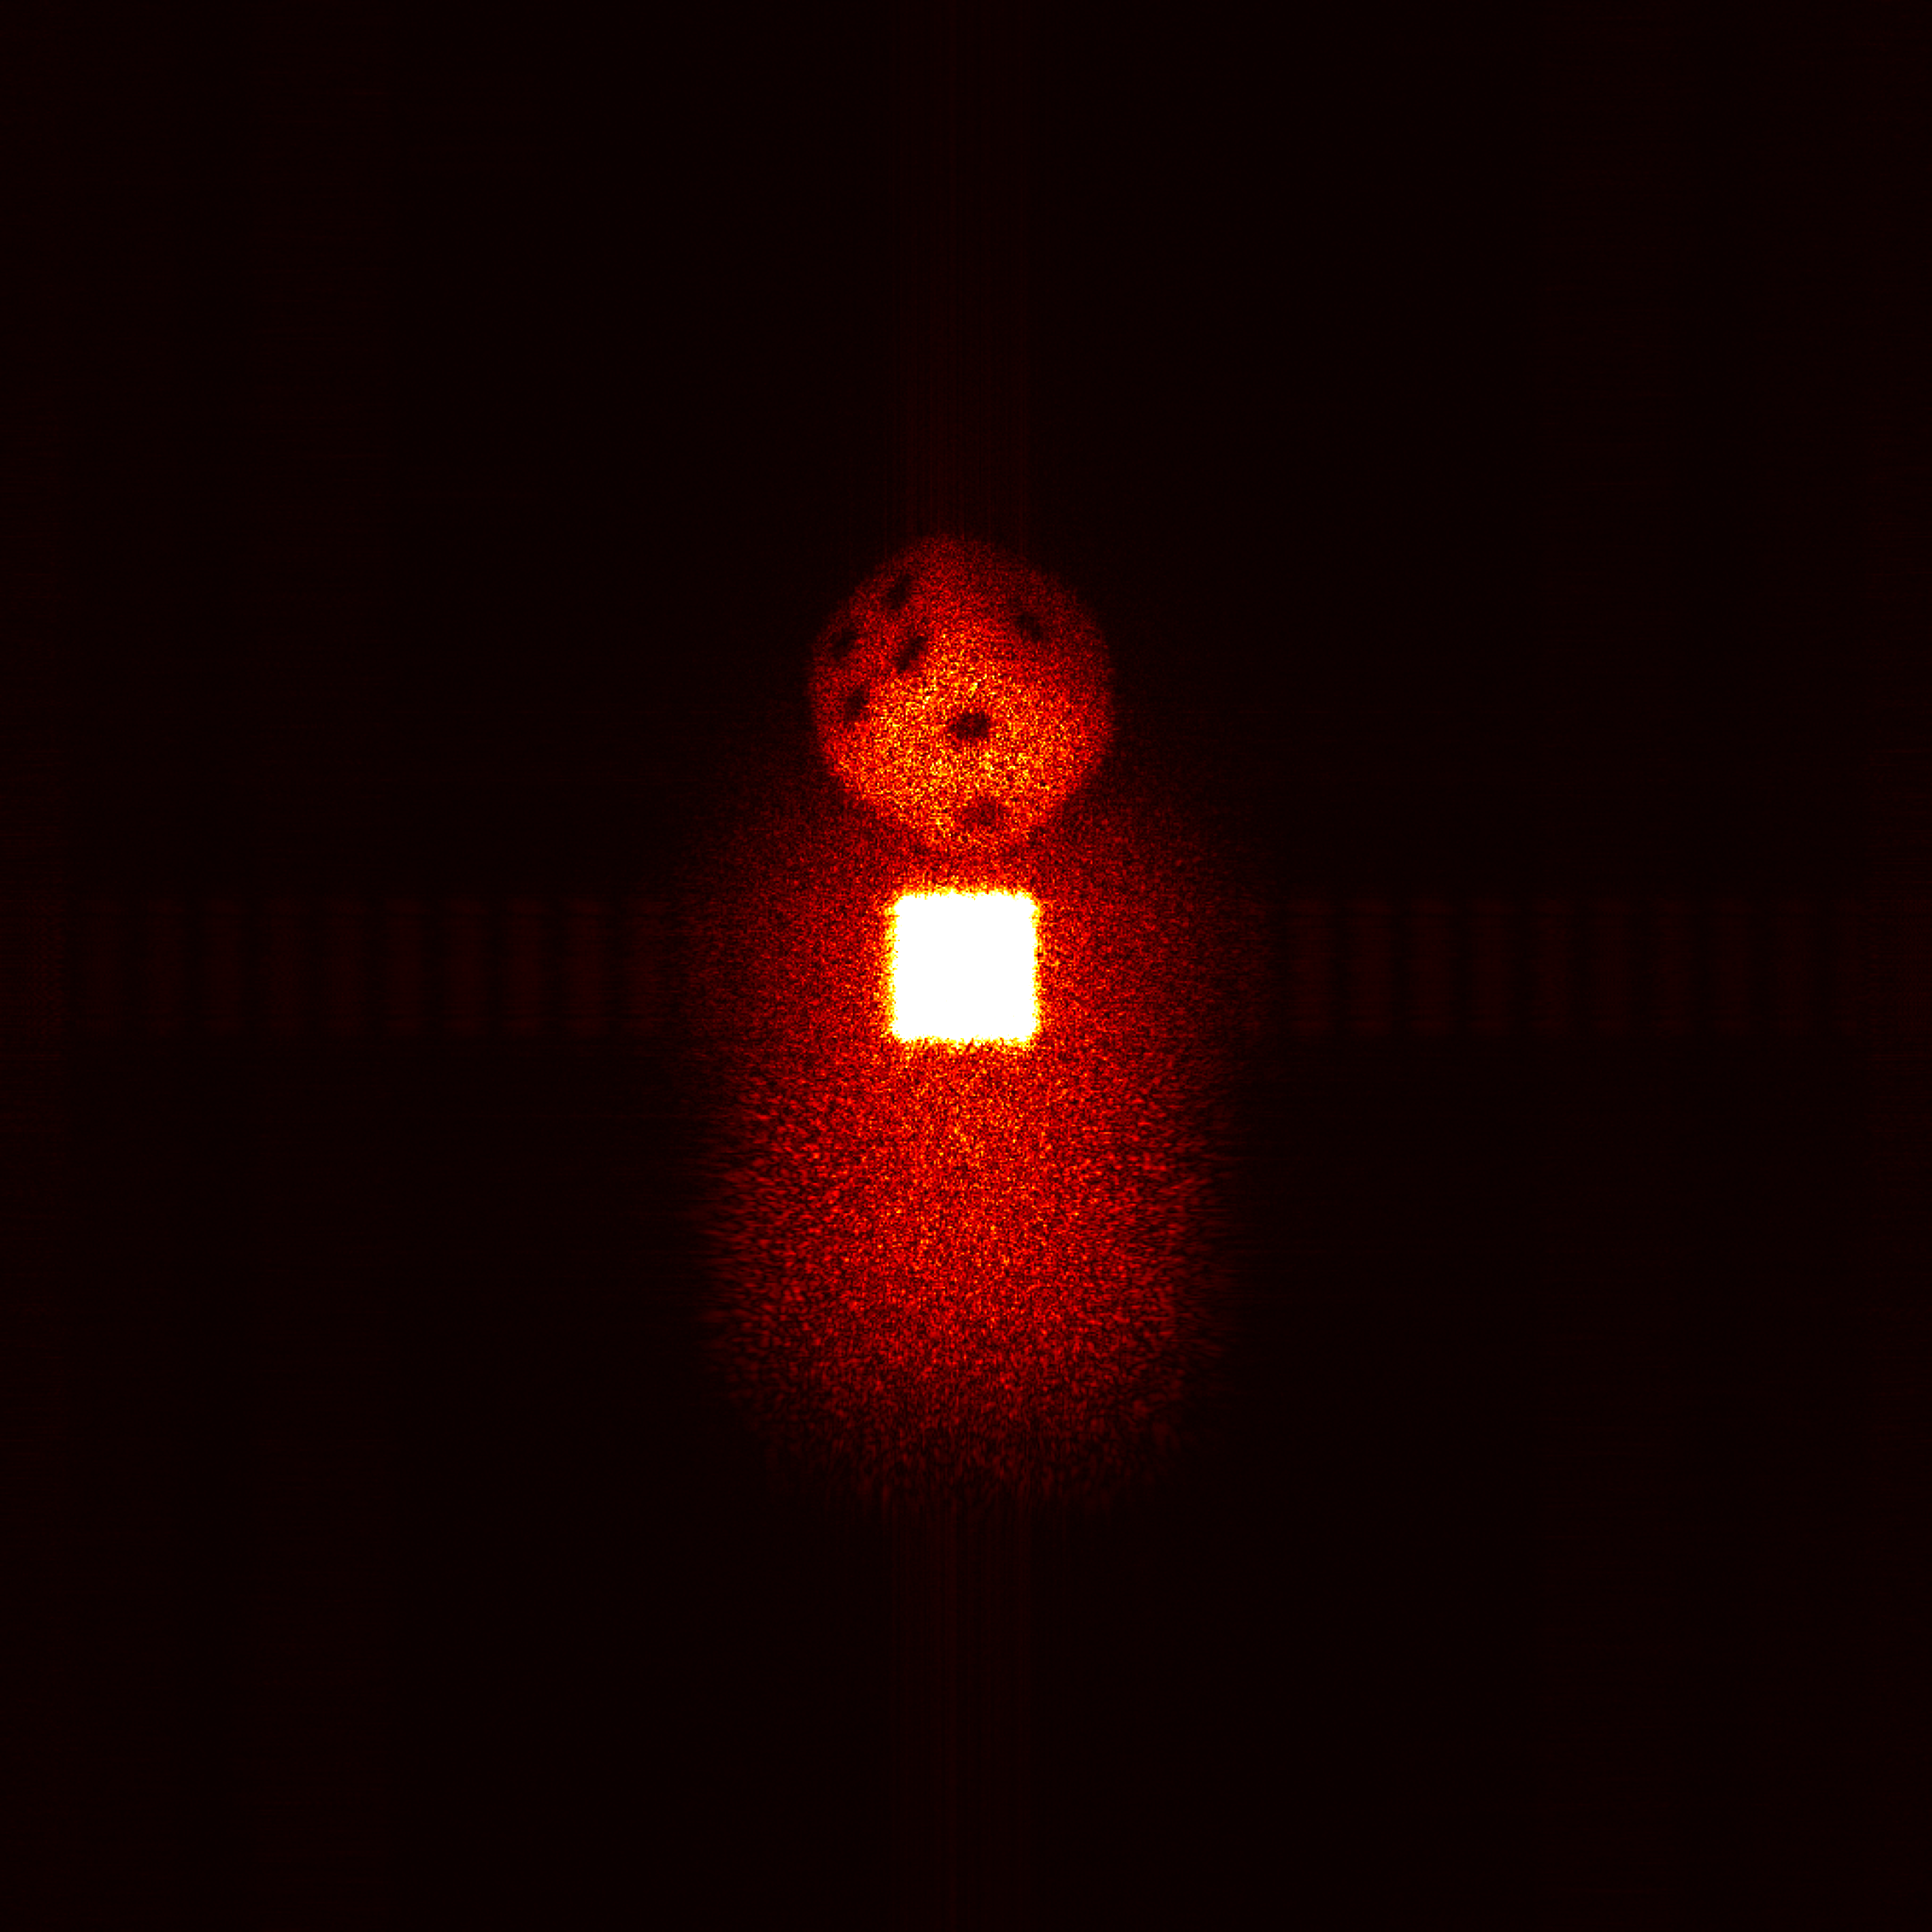
\includegraphics[width=0.3\textwidth]{attachments/dice_reconstructed.png}
            }
            \label{fig.2}
            \caption{\textbf{Digital holography}}
        \end{figure}



%end---------------------Exp.3---------------------------%

\section{Data and code availability}
Data and code are available at \url{https://github.com/Zweig-Wong/SYSU-PHY-EXP}

\end{document}